\documentclass[12pt]{article}

\usepackage{sbc-template}
\usepackage[utf8]{inputenc}
\usepackage[T1]{fontenc}
\usepackage[brazil]{babel}
\usepackage{graphicx,url}
\usepackage{amsmath,amssymb}
\usepackage{booktabs}
\usepackage{tabularx}
\usepackage{float}
\usepackage{placeins}
\usepackage{tikz}
\usetikzlibrary{positioning}

\sloppy
\raggedbottom

\title{REMG: a rede de distribuição de energia de Belo Horizonte\\ modelada e analisada como grafo}

\author{Davi Lage\inst{1}, Isaias Alves\inst{1}, Laura Noronha Lara\inst{1}, Lucas Spiazzi\inst{1}}

\address{Pontifícia Universidade Católica de Minas Gerais (PUC Minas)\\
  Belo Horizonte -- MG -- Brasil}

\begin{document}

\maketitle

\begin{resumo}
Este artigo apresenta o REMG, uma ferramenta que modela a rede de distribuição de energia de Belo Horizonte como um grafo desenhado sobre o mapa real da cidade. As linhas de alta tensão e as subestações vêm do OpenStreetMap, e a rede de distribuição é gerada sobre as ruas com um Dijkstra de várias fontes. Sobre esse grafo, um núcleo em Python responde a quatro perguntas de operação: quanto de energia chega aos consumidores (fluxo máximo de Dinic), onde estão os gargalos (corte mínimo), quem fica sem luz quando uma linha ou subestação falha (BFS) e como religar essas áreas por chaves de manobra (Dijkstra seguido de um novo cálculo de fluxo). Pontes e pontos de articulação saem de um Tarjan iterativo. As 27 comparações concluídas com o NetworkX deram respostas iguais; o núcleo foi mais rápido em 25 delas. O Edmonds-Karp na rede elétrica excedeu o limite de 120 segundos.
\end{resumo}

% =====================================================================
\section{Introdução}

Uma rede de distribuição de energia leva eletricidade das \textbf{subestações} até os \textbf{consumidores} por cabos de \textbf{capacidade limitada}. No dia a dia, a operadora precisa se preocupar com quatro questões: (i) quanto de energia consegue entregar e por onde ela passa; (ii) quais cabos limitam a entrega, ou seja, onde estão os gargalos; (iii) se uma linha ou uma subestação cair, quem fica sem luz; e (iv) como religar quem ficou sem luz por outro caminho.

As quatro perguntas são problemas clássicos de grafos. A primeira é um problema de \textbf{fluxo máximo}~\cite{ford1956}; a segunda é o \textbf{corte mínimo} associado a esse fluxo; a terceira é um problema de \textbf{alcançabilidade}, resolvido por busca em largura; e a quarta é um problema de \textbf{caminho mínimo} com restrições, seguido de uma nova verificação de fluxo. A esse conjunto somamos a identificação de \textbf{pontes} e \textbf{pontos de articulação}~\cite{tarjan1972}, que mostram os pontos da rede em que uma única falha separa uma área do resto.

Este trabalho, desenvolvido para a disciplina de Teoria de Grafos e Computabilidade (tema 4, distribuição de energia), aplica esses algoritmos à cidade inteira de Belo Horizonte. A ideia escolhida pelo grupo foi trabalhar sobre o mapa real: a alta tensão vem do OpenStreetMap~\cite{osm}, a rede de distribuição é gerada sobre as ruas reais, e o resultado é desenhado em cima do mapa, com o fluxo animado, os gargalos marcados e a simulação de falhas.

A regra principal do trabalho é que \textbf{o grafo e todos os algoritmos são implementados à mão}, sem biblioteca de grafos. O NetworkX~\cite{hagberg2008} aparece apenas no benchmark, como gabarito de corretude e como referência de desempenho. O núcleo usa somente a biblioteca padrão do Python, e nem a fila de prioridade da biblioteca (\texttt{heapq}) é usada: a heap binária também foi escrita pelo grupo.

As seções seguintes tratam dos dados (\ref{sec:dados}), da modelagem (\ref{sec:modelagem}), dos algoritmos (\ref{sec:algoritmos}), da arquitetura e das telas (\ref{sec:arquitetura}), dos resultados (\ref{sec:resultados}), das limitações (\ref{sec:limitacoes}), do processo, do uso de IA e das responsabilidades (\ref{sec:processo}) e da conclusão (\ref{sec:conclusao}).

% =====================================================================
\section{Dados}
\label{sec:dados}

\subsection{O que existe no OpenStreetMap de Belo Horizonte}

Os dados foram baixados uma única vez da Overpass API, restringindo a consulta ao município pelo código do IBGE (3106200). A restrição pelo nome não basta, uma vez que a primeira tentativa trouxe junto uma linha de transmissão de uma cidade em Moçambique. A Tabela~\ref{tab:osm} resume o que foi extraído.

\begin{table}[ht]
\centering
\caption{Dados de Belo Horizonte extraídos do OpenStreetMap e gravados em CSV.}
\label{tab:osm}
\begin{tabular}{lrl}
\toprule
\textbf{Camada} & \textbf{Quantidade} & \textbf{Uso no sistema} \\
\midrule
Pontos de rua (cruzamentos e pontas) & 35.829 & vértices da rede \\
Trechos de rua & 53.230 & base da rede gerada \\
Subestações (\texttt{power=substation}) & 25 & fontes de energia \\
Linhas de alta tensão (\texttt{power=line}) & 60 & ligação real entre subestações \\
Regionais administrativas & 9 & desenho e filtro \\
\bottomrule
\end{tabular}
\end{table}

O OSM tem a alta tensão de Belo Horizonte, mas quase nada da distribuição: apenas uma linha de baixa tensão, um transformador e seis postes. Por isso a rede de distribuição é gerada (Seção~\ref{sec:geracao}). As ruas, por outro lado, estão completas e servem de traçado para os cabos, como acontece na vida real.

\subsection{Caminho dos dados}

A ferramenta \texttt{tools/prep\_osm} lê o arquivo bruto do OSM (que fica fora do repositório) e grava cinco arquivos CSV em \texttt{data/bh/}: pontos, trechos de rua, subestações, linhas de alta tensão e regionais. O comprimento de cada trecho, em metros, é calculado pela fórmula de Haversine. Essa ferramenta pode usar bibliotecas, mas \textbf{não monta grafo nenhum}: ela só extrai listas. Juntar os pontos num grafo, gerar a rede de distribuição e rodar qualquer busca é trabalho do núcleo feito à mão. Os dados do OSM estão sob a licença ODbL, e a atribuição \textquotedblleft{}\copyright{} OpenStreetMap contributors\textquotedblright{} aparece no mapa.

\subsection{Rede de distribuição sintética}
\label{sec:geracao}

A rede de distribuição é gerada no núcleo, a cada vez que o sistema liga, de forma que a mesma entrada sempre gera a mesma rede:

\begin{enumerate}
  \item cada subestação de distribuição é ligada ao ponto de rua mais próximo, o \emph{ponto raiz};
  \item um \textbf{Dijkstra com várias fontes}~\cite{dijkstra1959}, partindo de todas as raízes ao mesmo tempo e usando o comprimento da rua como peso, divide a cidade em \textbf{áreas de atendimento}: cada ponto fica com a subestação mais próxima pelas ruas;
  \item a árvore de caminhos mínimos de cada área vira o \textbf{alimentador} (rede radial, como nas redes reais); a rua que liga áreas de subestações diferentes vira uma \textbf{chave de manobra}, normalmente aberta; as demais ruas ficam sem cabo;
  \item a demanda de cada ponto é proporcional ao comprimento de rua ao seu redor (0,05~kVA por metro, metade de cada rua para cada ponta); a capacidade de cada cabo é a demanda que passa por ele multiplicada por um fator sorteado entre 1,1 e 2,5, com semente fixa. Com fator abaixo de cerca de 1,11, o uso do cabo passa de 90\% e ele vira gargalo; acima de cerca de 1,67, o uso fica abaixo de 60\%;
  \item \textbf{socorro}: em cada área, a chave mais curta da fronteira é a que a rota alternativa fecha quando a subestação cai. Essa chave, os cabos do caminho até as duas raízes e a subestação vizinha são dimensionados para aguentar a área socorrida inteira. Cada subestação recebe 1,2 vez a soma da demanda da sua área com a da maior área que ela socorre.
\end{enumerate}

Como os cabos de cada alimentador formam uma árvore, a demanda que passa pelo cabo que chega a um ponto $v$ é a soma das demandas da subárvore de $v$. Essa soma é feita em $O(V \log V)$, percorrendo os pontos em ordem decrescente de distância à raiz: quando um ponto é visitado, todos os seus filhos já foram somados.

% =====================================================================
\section{Modelagem}
\label{sec:modelagem}

\subsection{O grafo}

A Tabela~\ref{tab:modelo} mostra como cada elemento da rede elétrica vira parte do grafo. Todas as capacidades usam uma única unidade, o kVA. Internamente, o núcleo trabalha com inteiros em VA para que o fluxo seja exato.

\begin{table}[ht]
\centering
\caption{Elementos da rede elétrica e sua representação no grafo.}
\label{tab:modelo}
\begin{tabularx}{\textwidth}{lXX}
\toprule
\textbf{Elemento} & \textbf{No grafo} & \textbf{Atributos} \\
\midrule
Subestação & vértice & capacidade, nome, ponto raiz \\
Ponto de suprimento & vértice & entrada de alta tensão na divisa \\
Ponto de rua & vértice & latitude, longitude, demanda \\
Trecho (cabo) & aresta não direcionada & capacidade, comprimento, falha \\
Chave de manobra & aresta não direcionada & como o trecho, mais \emph{aberta} \\
Linha de alta tensão & aresta não direcionada & tensão, capacidade \\
Super-fonte $S$ & vértice virtual & $S \to$ pontos de suprimento, capacidade infinita \\
Super-sorvedouro $T$ & vértice virtual & ponto $\to T$, capacidade = demanda \\
Transformação & aresta subestação $\to$ raiz & capacidade = capacidade da subestação \\
\bottomrule
\end{tabularx}
\end{table}

A super-fonte e o super-sorvedouro transformam o problema de várias fontes e vários consumidores num único problema de fluxo $S$--$T$. As linhas de alta tensão que cruzam a divisa do município viram \textbf{pontos de suprimento}, ligados a $S$; as pontas de linha que caem a menos de 200~m de uma subestação se ligam a ela. A aresta de \emph{transformação}, da subestação até o ponto raiz, é a que limita a capacidade da subestação no fluxo.

Uma \textbf{chave aberta} ou um \textbf{trecho em falha} continuam no grafo, mas com capacidade zero: nada passa por eles. Cada cenário monta uma nova instância do grafo com a mesma topologia e os mesmos identificadores de aresta, alterando as capacidades conforme as falhas e as chaves fechadas.

\textbf{Plano B para a alta tensão incompleta.} O OSM não tem a alta tensão completa: em Belo Horizonte, 5 das 18 subestações de distribuição (Centro, Carlos Prates, Serrano, Barro Preto e Calafate) não alcançam nenhum ponto de suprimento andando pelas linhas de alta tensão. Sem tratamento, as áreas delas ficariam apagadas sem falha nenhuma. A regra adotada é: a subestação que não alcança nenhum ponto de suprimento liga direto em $S$. Essas subestações ficam registradas em \texttt{RedeEletrica.subestacoes\_sem\_alta\_tensao}.

\subsection{Representação na memória}

O grafo usa uma \textbf{lista de adjacência em vetores} (\emph{forward-star}): \texttt{head[v]} guarda o primeiro arco que sai de $v$, \texttt{prox[e]} o próximo arco do mesmo vértice, \texttt{para[e]} o destino e \texttt{cap[e]} a capacidade. Cada aresta não direcionada vira \textbf{dois arcos em par}, $e$ e $e \oplus 1$ (o par difere só no último bit). O mesmo par serve de aresta reversa no grafo residual do fluxo, sem estrutura extra. Os vértices são inteiros $0..V-1$; o identificador do OSM fica num mapa à parte (por exemplo, \texttt{"t:678"} $\leftrightarrow$ arco 1356), mantido pelo domínio.

\subsection{Diagramas UML}

O diagrama de casos de uso (Figura~\ref{fig:casos}) mostra o que o operador faz na ferramenta. Simular uma falha sempre inclui calcular quem ficou sem energia, e a rota alternativa estende a simulação de falha.

\begin{figure}[!htbp]
\centering
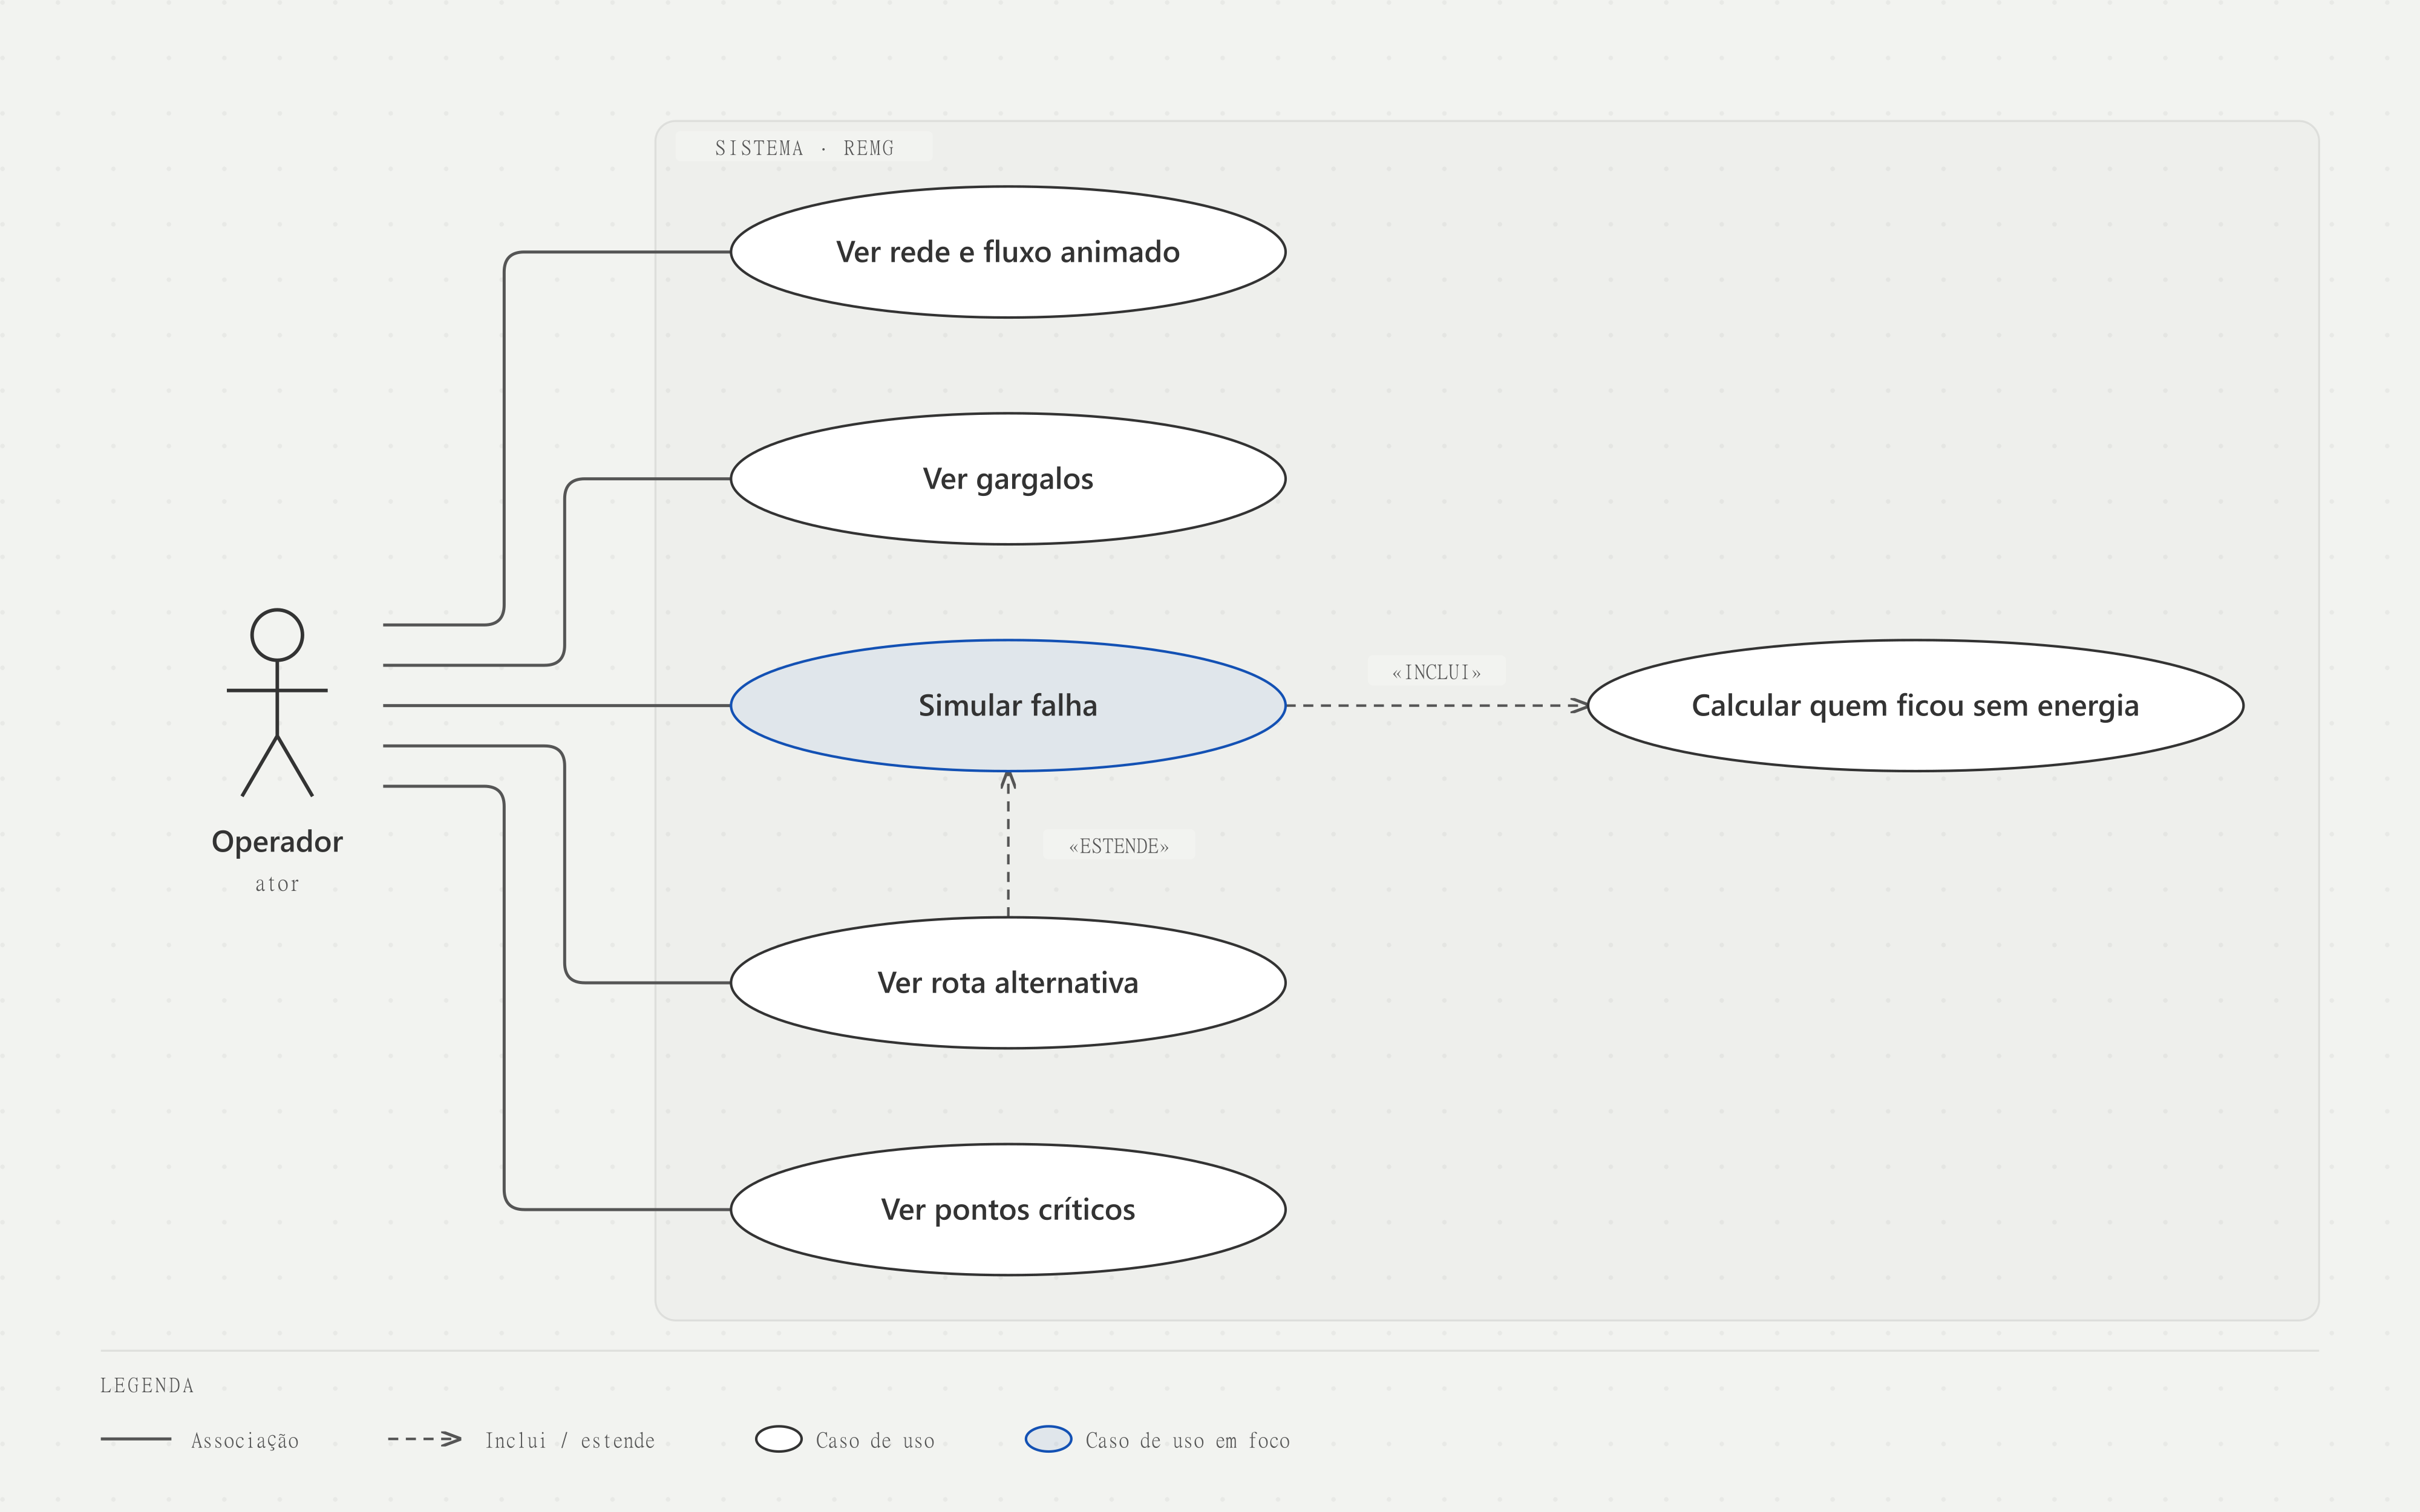
\includegraphics[width=.78\textwidth]{figuras/casos-de-uso.png}
\caption{Casos de uso na versão atual: rede e fluxo, gargalos, falhas, rota alternativa e pontos críticos.}
\label{fig:casos}
\end{figure}

\begin{figure}[!htbp]
\centering
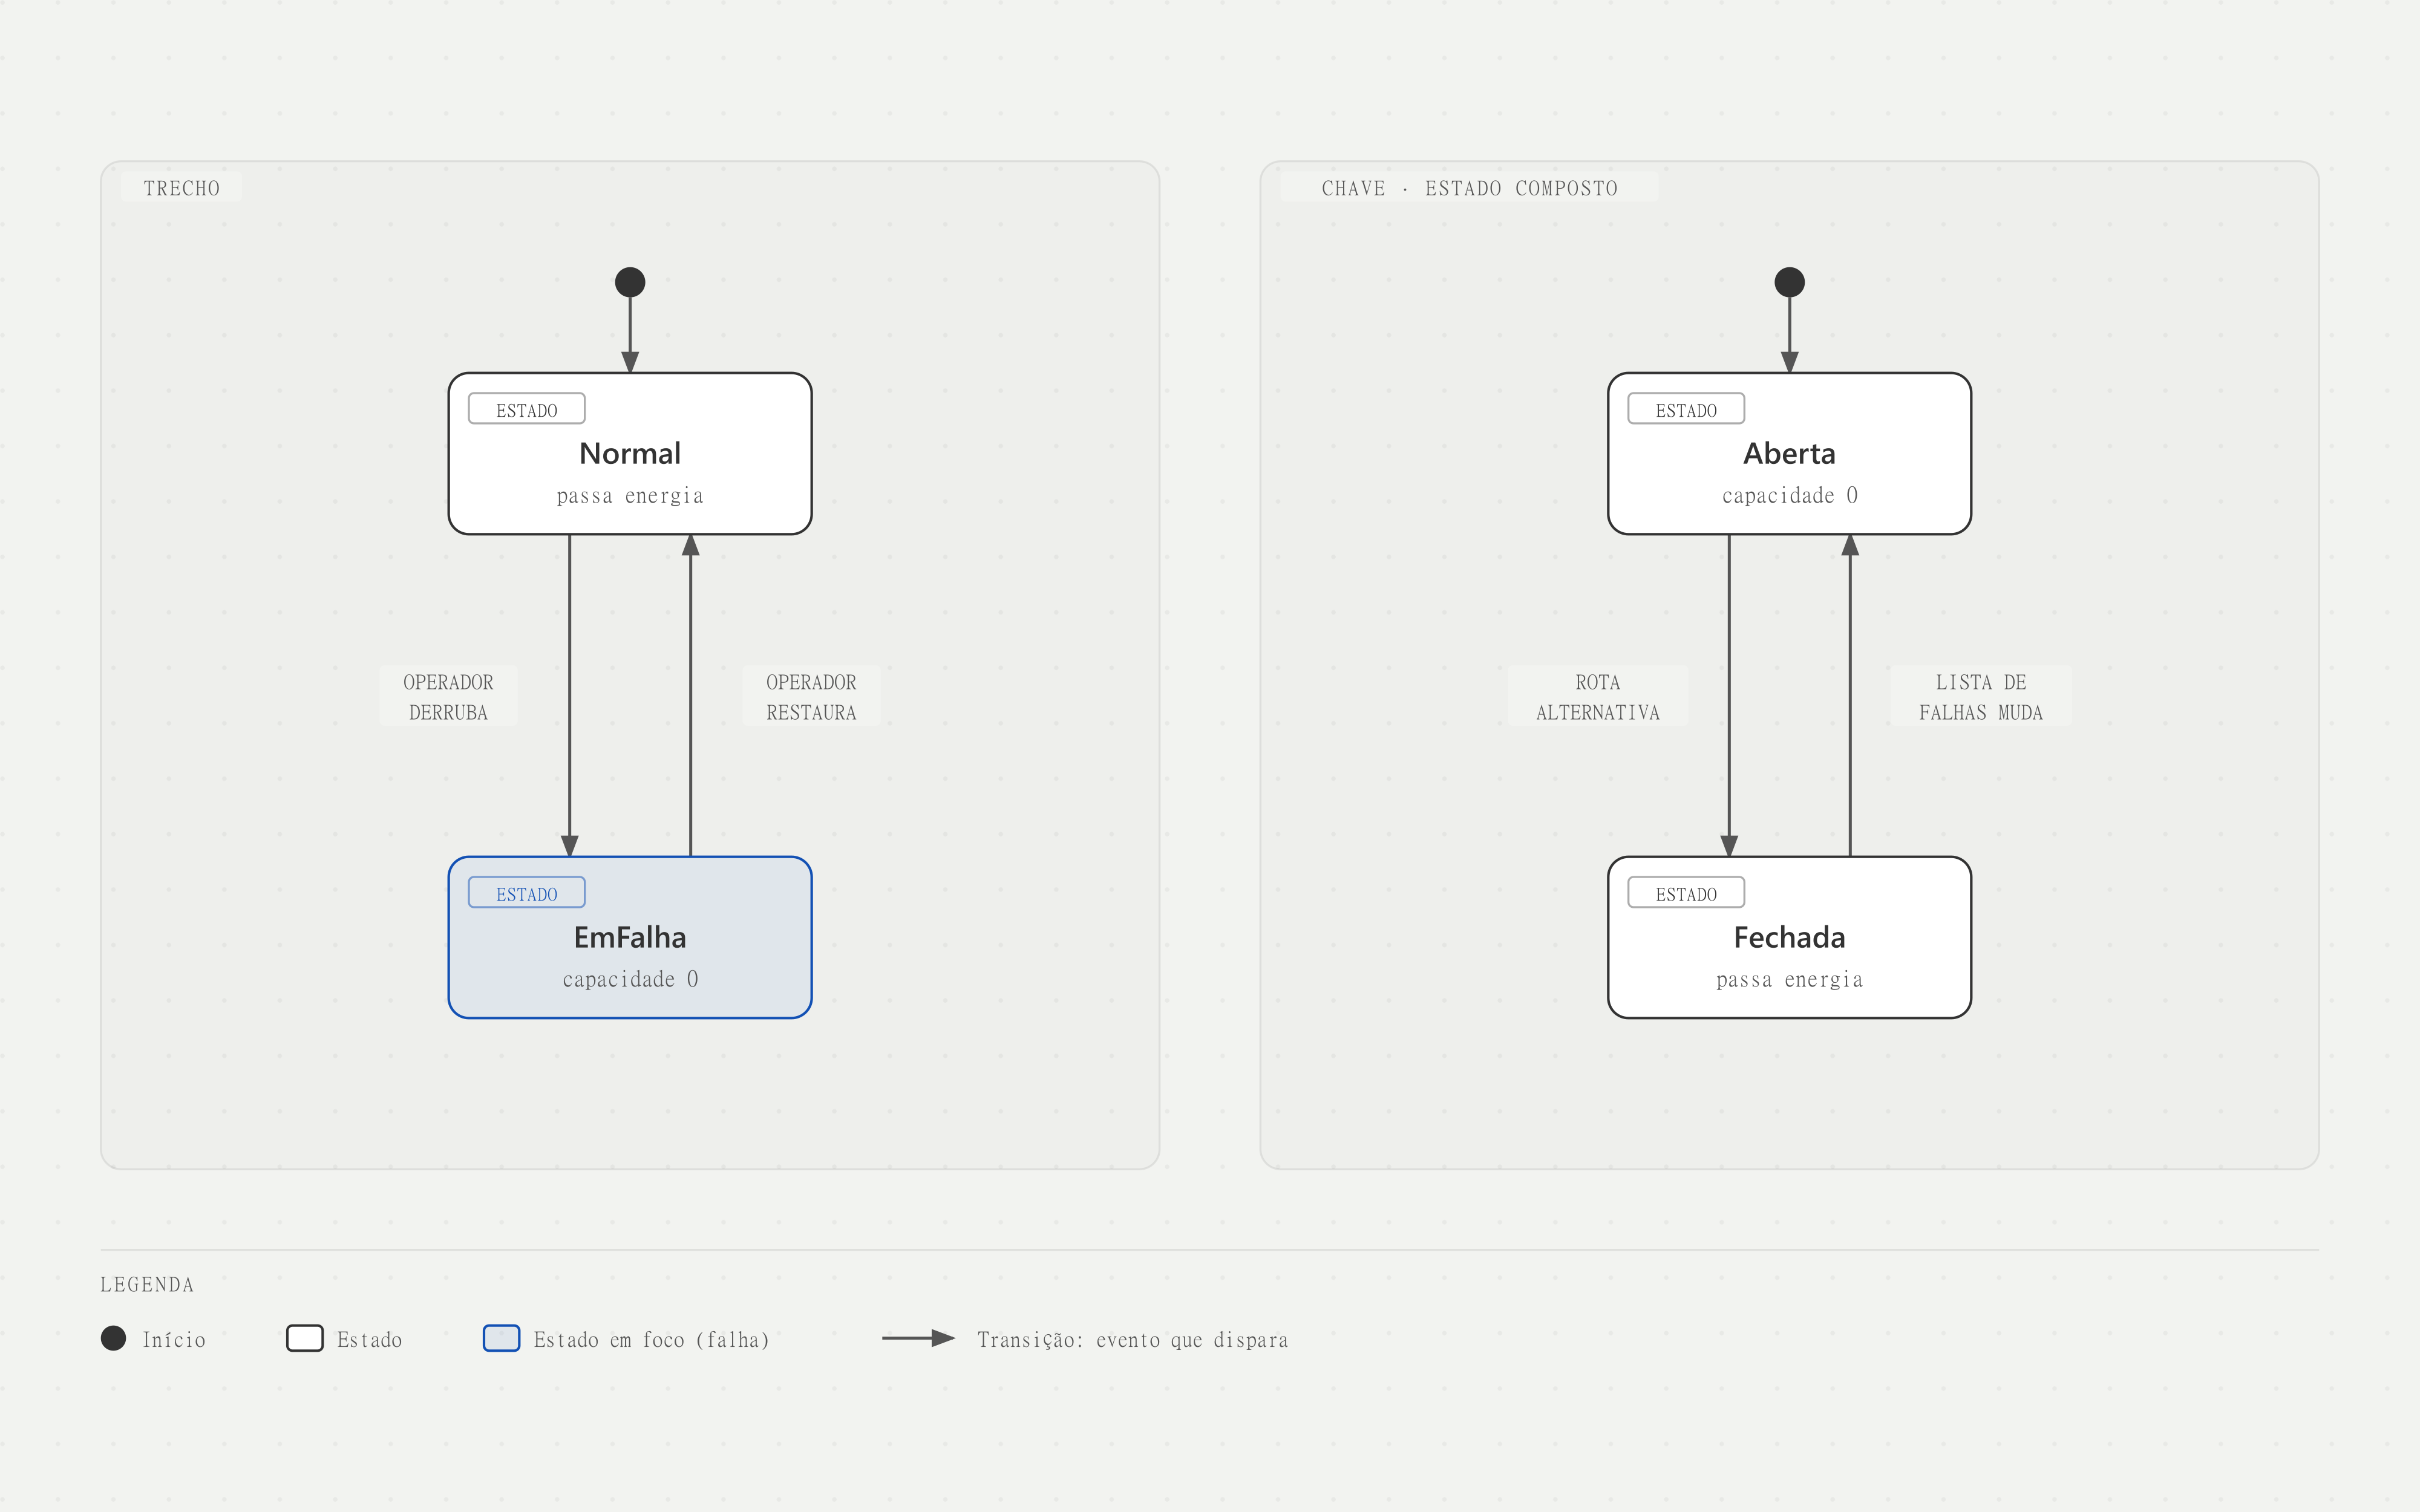
\includegraphics[width=.64\textwidth]{figuras/estados-trecho.png}
\caption{Estados de trechos e chaves. Uma falha ou chave aberta recebe capacidade zero nos cálculos.}
\label{fig:estados}
\end{figure}


Os diagramas desta revisão foram atualizados a partir dos SVGs do projeto, com a paleta da interface atual. O diagrama de classes do núcleo (Figura~\ref{fig:classes}) tem dois pacotes e inclui Alcance, HeapBinaria, UnionFind e PontoDeSuprimento. O pacote \texttt{grafo} é genérico e não sabe nada de energia: só conhece vértices, arestas e capacidades. O pacote \texttt{dominio} traduz subestações, trechos, chaves e falhas para o grafo, por meio de \texttt{RedeEletrica.montar\_grafo()}. \texttt{Dinic} e \texttt{EdmondsKarp} têm a mesma interface, o que permite trocar um pelo outro na mesma rede para compará-los.

\begin{figure}[!htbp]
\centering
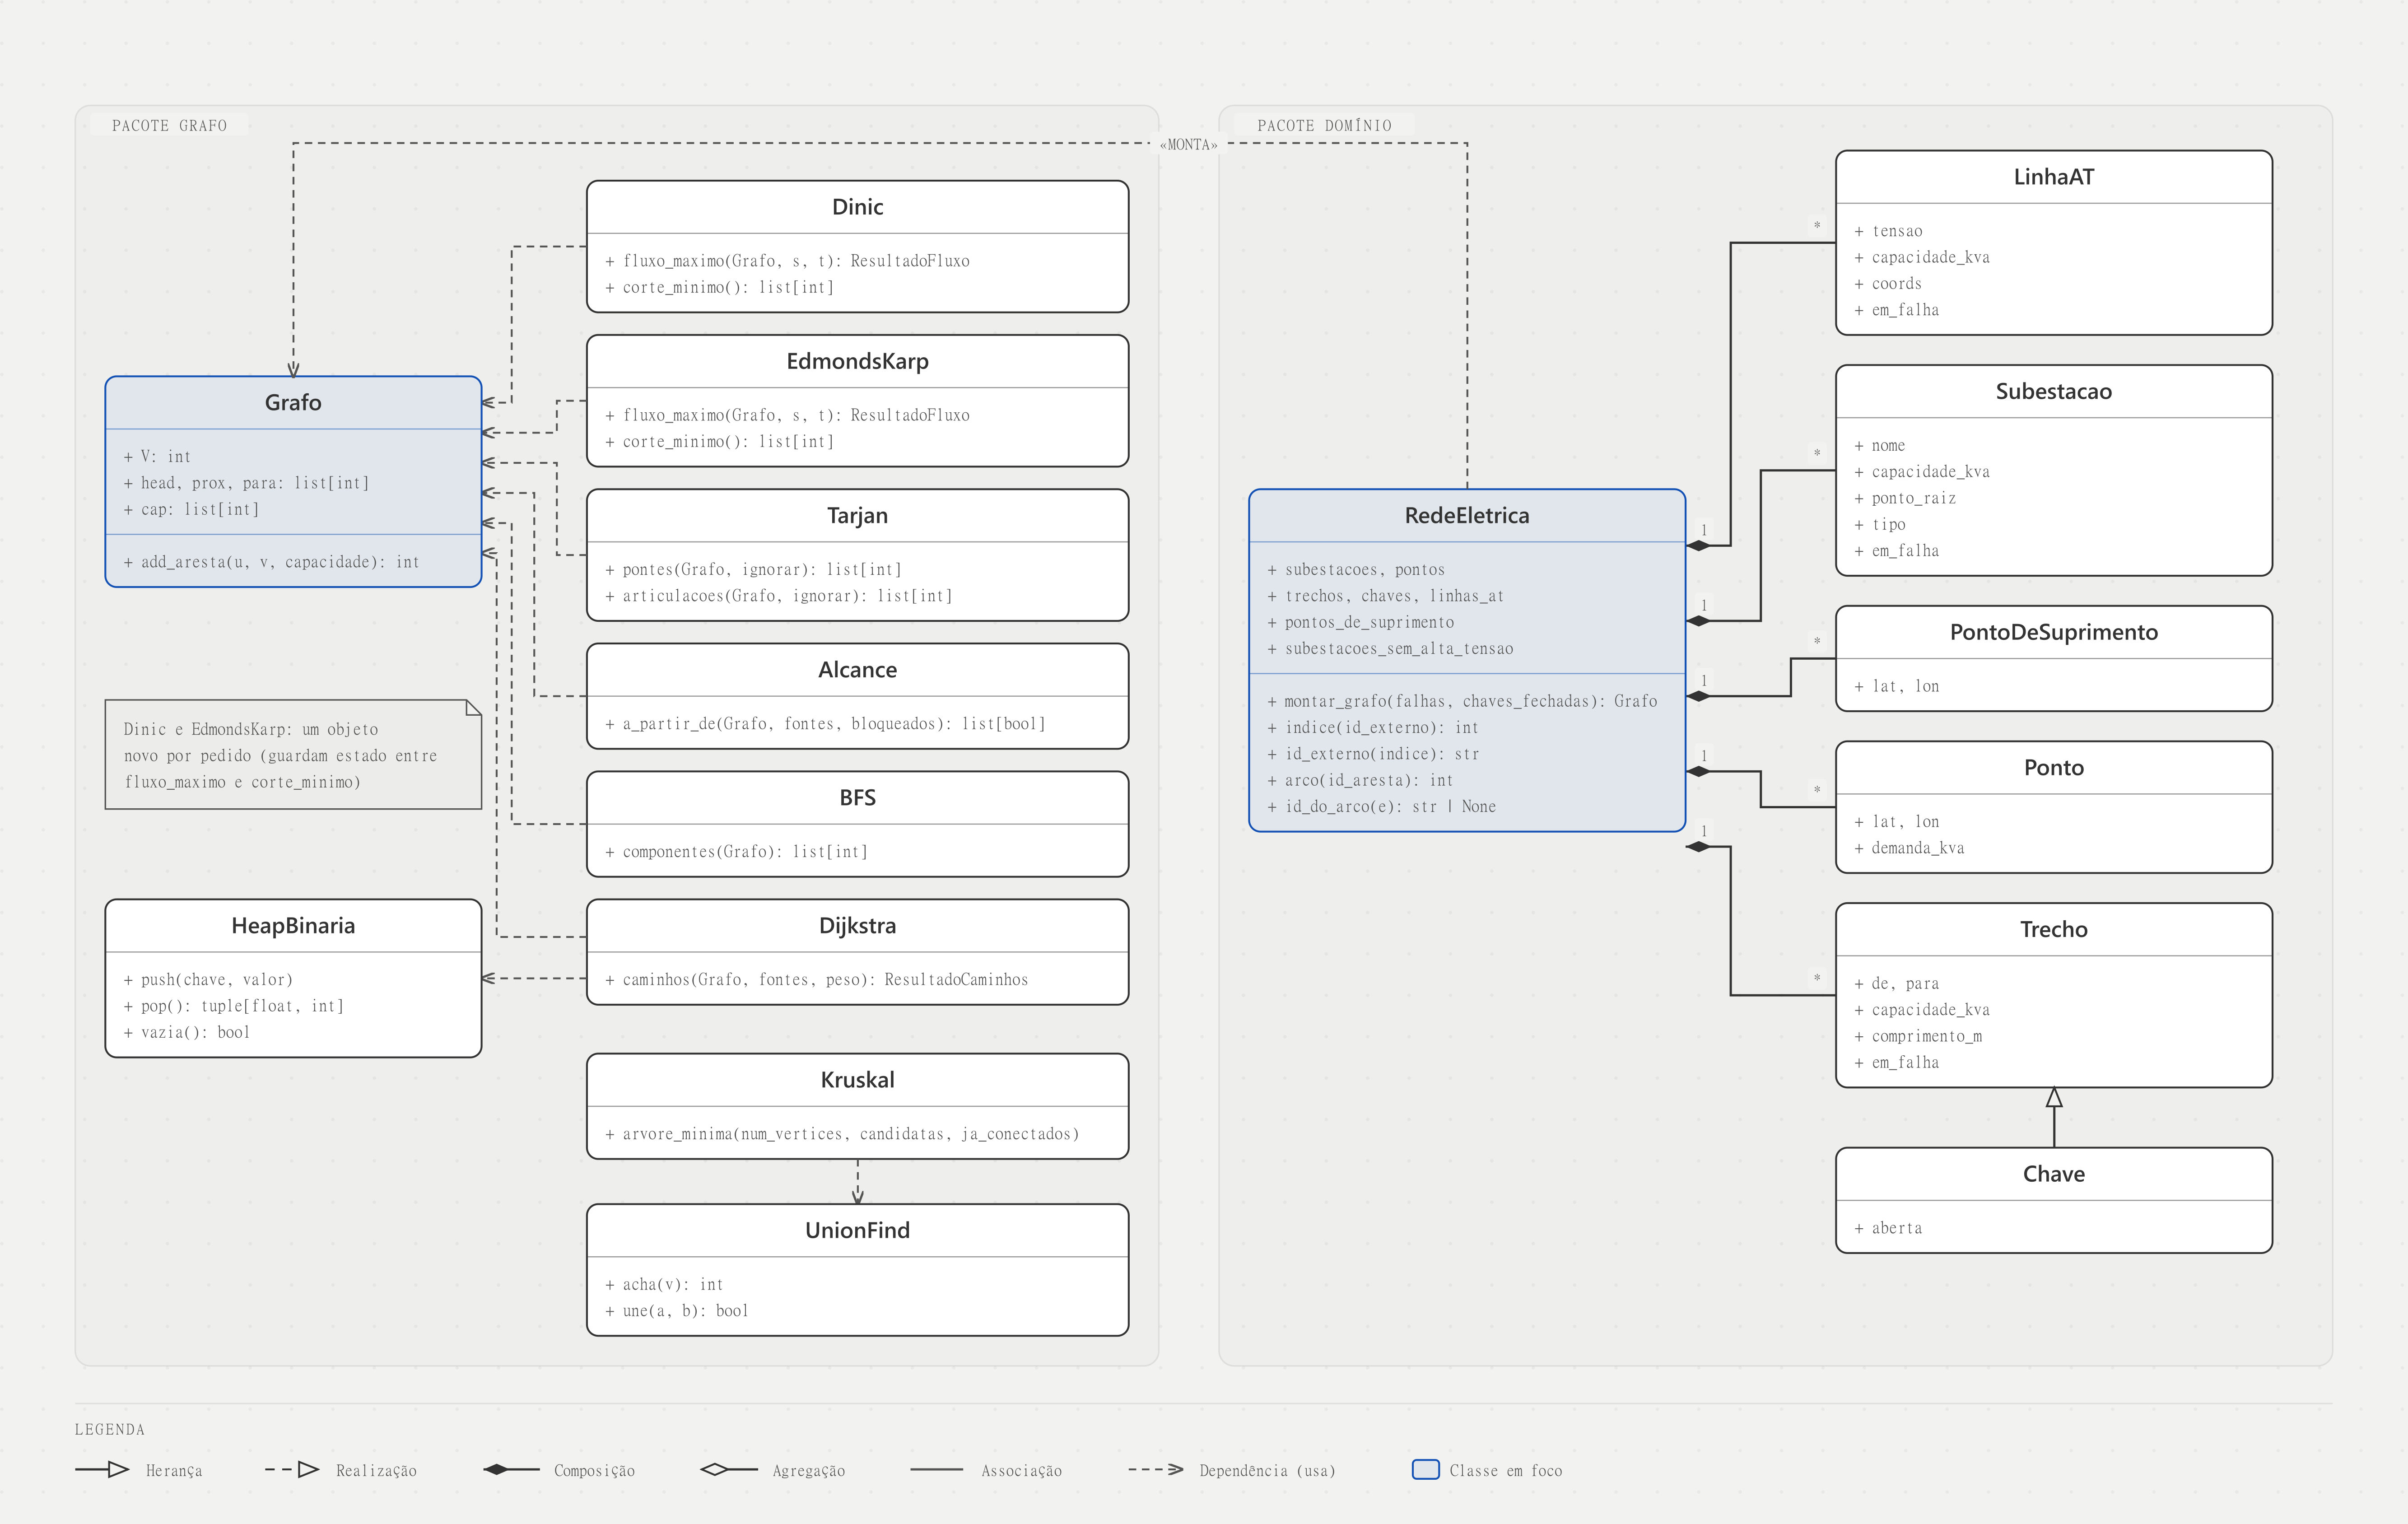
\includegraphics[width=.88\textwidth]{figuras/classes.png}
\caption{Diagrama de classes do núcleo: pacote de grafo genérico e pacote de domínio elétrico.}
\label{fig:classes}
\end{figure}

A Figura~\ref{fig:sequencia} mostra a sequência de uma simulação de falha. O operador clica em um trecho, o front envia a lista de falhas e de chaves fechadas, o caso de uso \texttt{SimularFalha} monta o grafo com as capacidades alteradas, roda uma busca em largura a partir de $S$ para achar quem ficou sem energia e roda o Dinic de novo para obter o fluxo novo. Os estados de trechos e chaves são mostrados na Figura~\ref{fig:estados}.

\begin{figure}[!htbp]
\centering
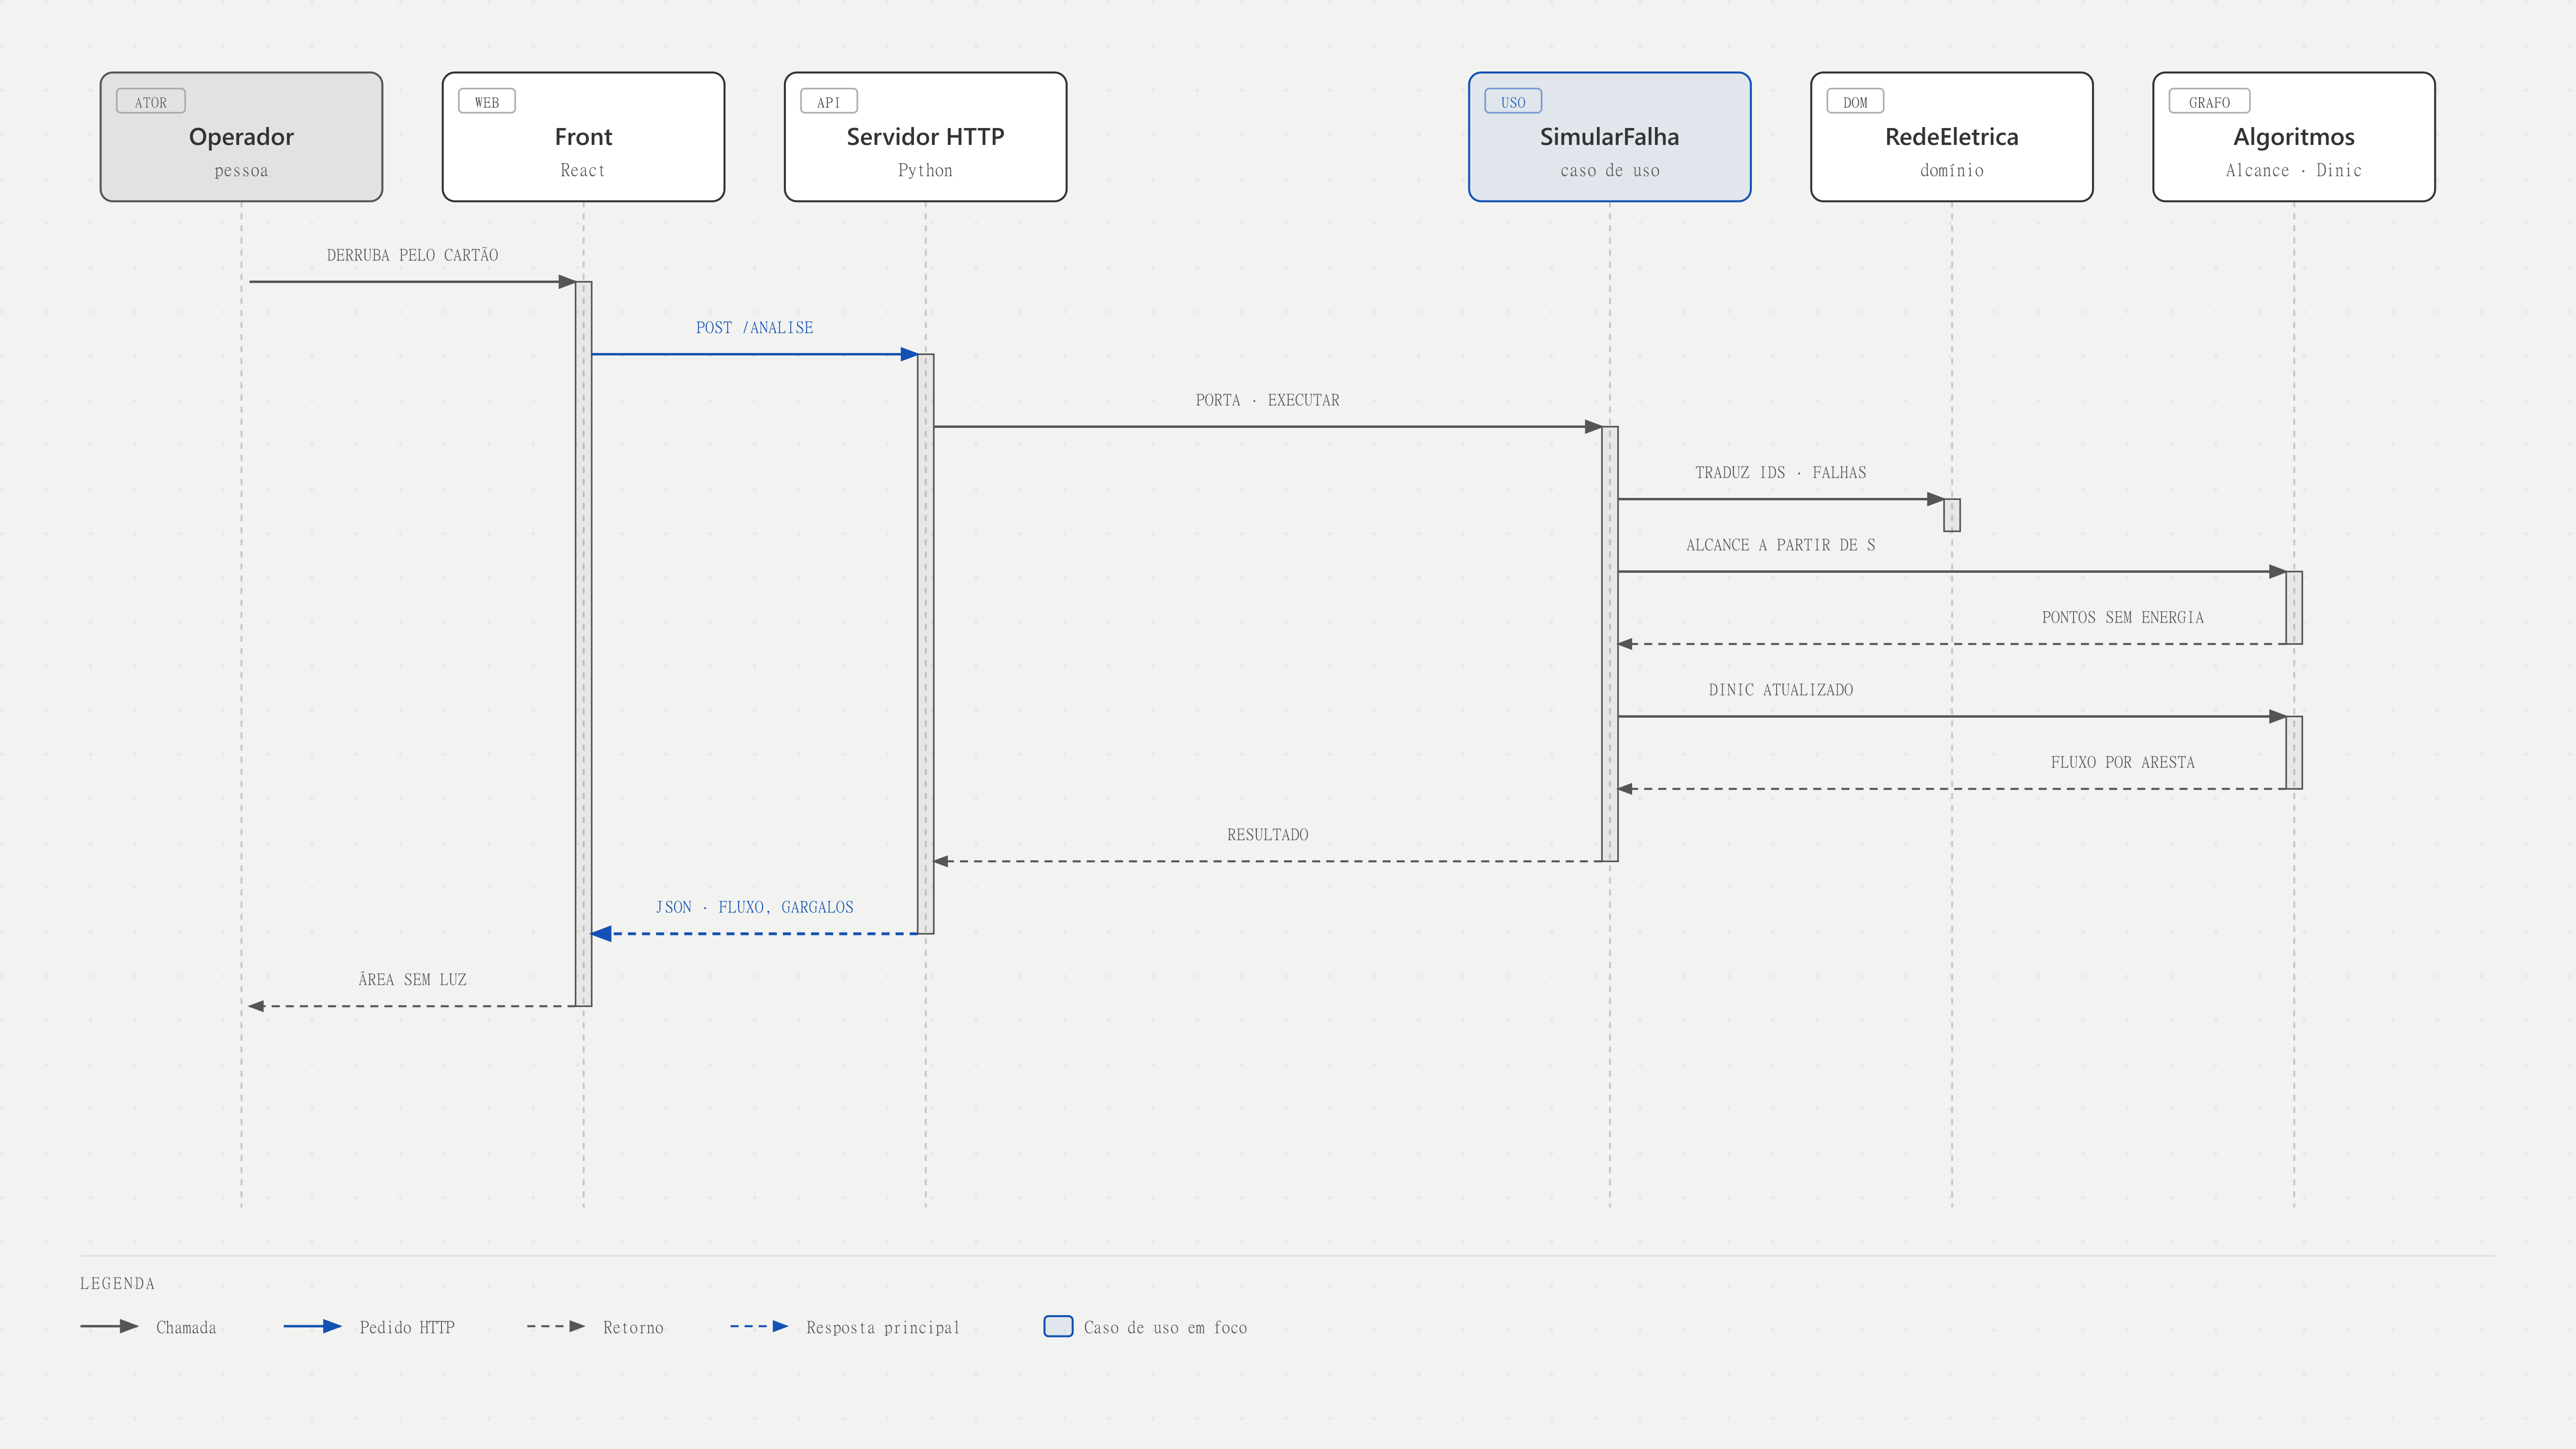
\includegraphics[width=.85\textwidth]{figuras/sequencia-simular-falha.png}
\caption{Diagrama de sequência de \textquotedblleft{}simular falha\textquotedblright{}.}
\label{fig:sequencia}
\end{figure}

% =====================================================================
\section{Algoritmos, complexidade e corretude}
\label{sec:algoritmos}

A Tabela~\ref{tab:algoritmos} associa cada pergunta ao algoritmo que a responde. Em todas as fórmulas, $V$ é o número de vértices, $E$ o de arestas e $A$ o número de rodadas de busca de rota, uma por chave fechada.

\begin{table}[H]
\centering\small
\caption{Perguntas, algoritmos e complexidade de pior caso.}
\label{tab:algoritmos}
\begin{tabularx}{\textwidth}{XlX}
\toprule
\textbf{Pergunta} & \textbf{Algoritmo} & \textbf{Complexidade} \\
\midrule
Gerar a rede de distribuição & Dijkstra com várias fontes & $O((V+E)\log V)$ \\
Quanto de energia chega, e por onde & Dinic (fluxo máximo) & $O(V^2 E)$ \\
Onde estão os gargalos & corte mínimo (BFS no residual) & $O(V+E)$ após o fluxo \\
Quem fica sem luz numa falha & BFS a partir de $S$ & $O(V+E)$ \\
Quais pontos são críticos & Tarjan iterativo & $O(V+E)$ \\
Como religar & Dijkstra por chaves + Dinic & $O(A(V+E)\log V)$ + fluxo \\
Comparação do fluxo & Edmonds-Karp & $O(V E^2)$ \\
Expandir a rede gastando menos cabo & Kruskal + \emph{union-find} & $O(E \log E)$ \\
\bottomrule
\end{tabularx}
\end{table}

\textbf{Sem recursão em grafo grande.} A rede de Belo Horizonte tem dezenas de milhares de vértices, e o Python interrompe a recursão por volta de mil chamadas. Por isso a busca em profundidade do Dinic e o Tarjan são \textbf{iterativos}, com pilha própria.

\subsection{Dijkstra com várias fontes e heap binária}

Todas as fontes entram na fila com distância zero; a cada passo sai o vértice de menor distância e suas arestas são relaxadas. O resultado guarda, para cada vértice, a distância, o arco pai e a fonte que o alcançou. A fila de prioridade é uma \textbf{heap binária feita à mão}, com \emph{push} e \emph{pop} em $O(\log n)$. Ela aceita entradas repetidas do mesmo vértice e descarta as velhas na saída (\emph{lazy deletion}), o que evita a operação de diminuir chave.

\subsection{Fluxo máximo de Dinic e corte mínimo}

O algoritmo de Dinic~\cite{dinic1970} repete duas fases até não haver mais caminho de $S$ a $T$ no grafo residual: (1) uma BFS a partir de $S$ calcula o \textbf{nível} de cada vértice; (2) buscas em profundidade enviam um \textbf{fluxo bloqueante} usando só arcos que sobem exatamente um nível, com um ponteiro por vértice que lembra o próximo arco a tentar. Cada fase custa $O(VE)$ e há no máximo $V$ fases, o que dá $O(V^2E)$ no pior caso; em redes como a nossa, quase em árvore, o número de fases é muito menor.

A última BFS do Dinic, que não encontra mais caminho até $T$, já separa os vértices alcançáveis dos não alcançáveis no grafo residual. Os arcos que vão do primeiro conjunto ao segundo formam o \textbf{corte mínimo}, e, pelo teorema do fluxo máximo e corte mínimo~\cite{ford1956,cormen2009}, a soma das suas capacidades é igual ao fluxo máximo. Na ferramenta, um trecho é marcado como \textbf{gargalo} se está no corte mínimo \textbf{ou} se o seu uso (fluxo dividido pela capacidade) é de pelo menos 90\%. A primeira condição vem do algoritmo; a segunda é regra de negócio e mora no domínio.

\subsection{Falhas, pontos críticos e rota alternativa}

\textbf{Falha.} Os trechos e subestações em falha recebem capacidade zero. Uma BFS sai de $S$, sem atravessar o sorvedouro virtual $T$, para identificar inclusive a subestação que está de pé mas perdeu a alimentação de alta tensão; o ponto não visitado está \textbf{sem energia}. Em seguida o Dinic roda no grafo alterado.

\textbf{Pontos críticos.} Numa rede radial, quase todo trecho é ponte. A informação útil é \textbf{onde a chave de manobra não salva}: o Tarjan iterativo roda com todas as chaves fechadas, ignorando $S$ e $T$ (que ligariam tudo e esconderiam as pontes), e devolve as pontes e os pontos de articulação que continuam existindo.

\textbf{Rota alternativa.} (1) Os pontos sem energia são a entrada; (2) um Dijkstra com várias fontes parte de todos eles ao mesmo tempo, andando pelos trechos de pé e podendo atravessar chaves abertas, com o comprimento como peso; (3) o primeiro ponto com energia alcançado define o caminho, e as chaves desse caminho são as que devem ser fechadas; (4) o processo se repete até não sobrar ponto apagado alcançável. Por fim, o Dinic roda com essas chaves fechadas. Se a capacidade do caminho novo não der conta da carga, a resposta é um \textbf{religamento parcial}, com a demanda efetivamente religada.

\subsection{Edmonds-Karp e Kruskal}

O Edmonds-Karp~\cite{edmonds1972} e Dinic foram implementados com a mesma interface, para que os dois sejam comparados na mesma rede. O Kruskal~\cite{kruskal1956} com \emph{union-find} (compressão de caminho e união por tamanho) responde à pergunta extra de como expandir a rede gastando o mínimo de cabo, recebendo os componentes já conectados como ponto de partida.

\subsection{Como a precisão foi verificada}

A corretude foi verificada de três formas complementares.

\textbf{Grafos pequenos resolvidos à mão.} A pasta \texttt{docs/testes/} documenta exemplos pequenos para grafo e BFS, heap e Dijkstra, Dinic e Kruskal. Os testes automatizados cobrem também os demais algoritmos e casos de uso. A Figura~\ref{fig:exemplo} mostra um deles: duas subestações (1 e 2) e três pontos com demandas 4, 7 e 5. Só saem dos lados das subestações os trechos 1--3 (capacidade 8) e 2--4 (capacidade 5), então o fluxo não passa de 13. É possível chegar a 13, e os pontos pedem 16: sobram 3 de demanda sem atender. O corte mínimo esperado é $\{1\text{--}3, 2\text{--}4\}$, com soma $8+5=13$, igual ao fluxo, como diz o teorema. O teste automático confere exatamente esses valores.

\begin{figure}[ht]
\centering
\begin{tikzpicture}[
  v/.style={circle,draw,minimum size=7mm,inner sep=0pt,font=\small},
  lab/.style={font=\scriptsize,fill=white,inner sep=1pt},
  corte/.style={very thick,red!70!black}]
\node[v] (s) at (0,0) {$S$};
\node[v] (a) at (2,1) {1};
\node[v] (b) at (2,-1) {2};
\node[v] (p3) at (4.5,1) {3};
\node[v] (p4) at (4.5,-1) {4};
\node[v] (p5) at (7,1.3) {5};
\node[v] (t) at (9,0) {$T$};
\draw (s) -- node[lab]{50} (a);
\draw (s) -- node[lab]{50} (b);
\draw[corte] (a) -- node[lab]{8} (p3);
\draw[corte] (b) -- node[lab]{5} (p4);
\draw (p3) -- node[lab]{3} (p4);
\draw (p3) -- node[lab]{6} (p5);
\draw (p3) -- node[lab,pos=.3]{4} (t);
\draw (p4) -- node[lab]{7} (t);
\draw (p5) -- node[lab]{5} (t);
\end{tikzpicture}
\caption{Grafo de teste resolvido à mão. Os números são capacidades; as arestas em vermelho formam o corte mínimo (8+5=13 = fluxo máximo). As arestas para $T$ têm a capacidade igual à demanda do ponto.}
\label{fig:exemplo}
\end{figure}

\textbf{Gabarito do NetworkX.} O benchmark (Seção~\ref{sec:benchmark}) roda o núcleo e o NetworkX no mesmo grafo e compara as respostas: valor do fluxo máximo, distâncias do Dijkstra, componentes conexas, pontes, pontos de articulação e peso da árvore geradora mínima. Em todos os 27 casos que terminaram, as respostas foram iguais.

\textbf{Testes automatizados.} Na revisão de 22/11/2026, passaram 138 testes do núcleo, 25 do servidor HTTP, 13 da linha de comando, 192 do front, 23 da extração do OSM e 82 do verificador de processo: 473 testes nessas seis suítes. No Windows, a suíte do verificador foi executada com o \texttt{sh} do Git disponível no caminho de comandos. As mensagens de falha de rede nos testes do extrator são cenários simulados de erro e repetição.

% =====================================================================
\section{Arquitetura e ferramenta}
\label{sec:arquitetura}

\subsection{Arquitetura hexagonal}

O sistema segue a arquitetura hexagonal, ou de portas e adaptadores~\cite{cockburn2005} (Figura~\ref{fig:hexagono}). O núcleo em Python guarda todas as regras e é dividido em camadas cujas dependências só apontam para dentro: grafo genérico $\leftarrow$ domínio elétrico $\leftarrow$ portas $\leftarrow$ casos de uso. Há duas portas: \texttt{ServicoDeAnalise}, por onde entram os pedidos, e \texttt{FonteDeRede}, por onde chegam os dados. O servidor HTTP e a linha de comando são adaptadores de entrada; o leitor de CSV é o adaptador de saída. O núcleo é testado sem servidor nem arquivo. O front chega aos casos de uso pelo adaptador HTTP. A CLI é um ponto de montagem (exceção D22): no benchmark, lê o grafo e chama diretamente os algoritmos genéricos, sem executar a análise elétrica completa.

\begin{figure}[!htbp]
\centering
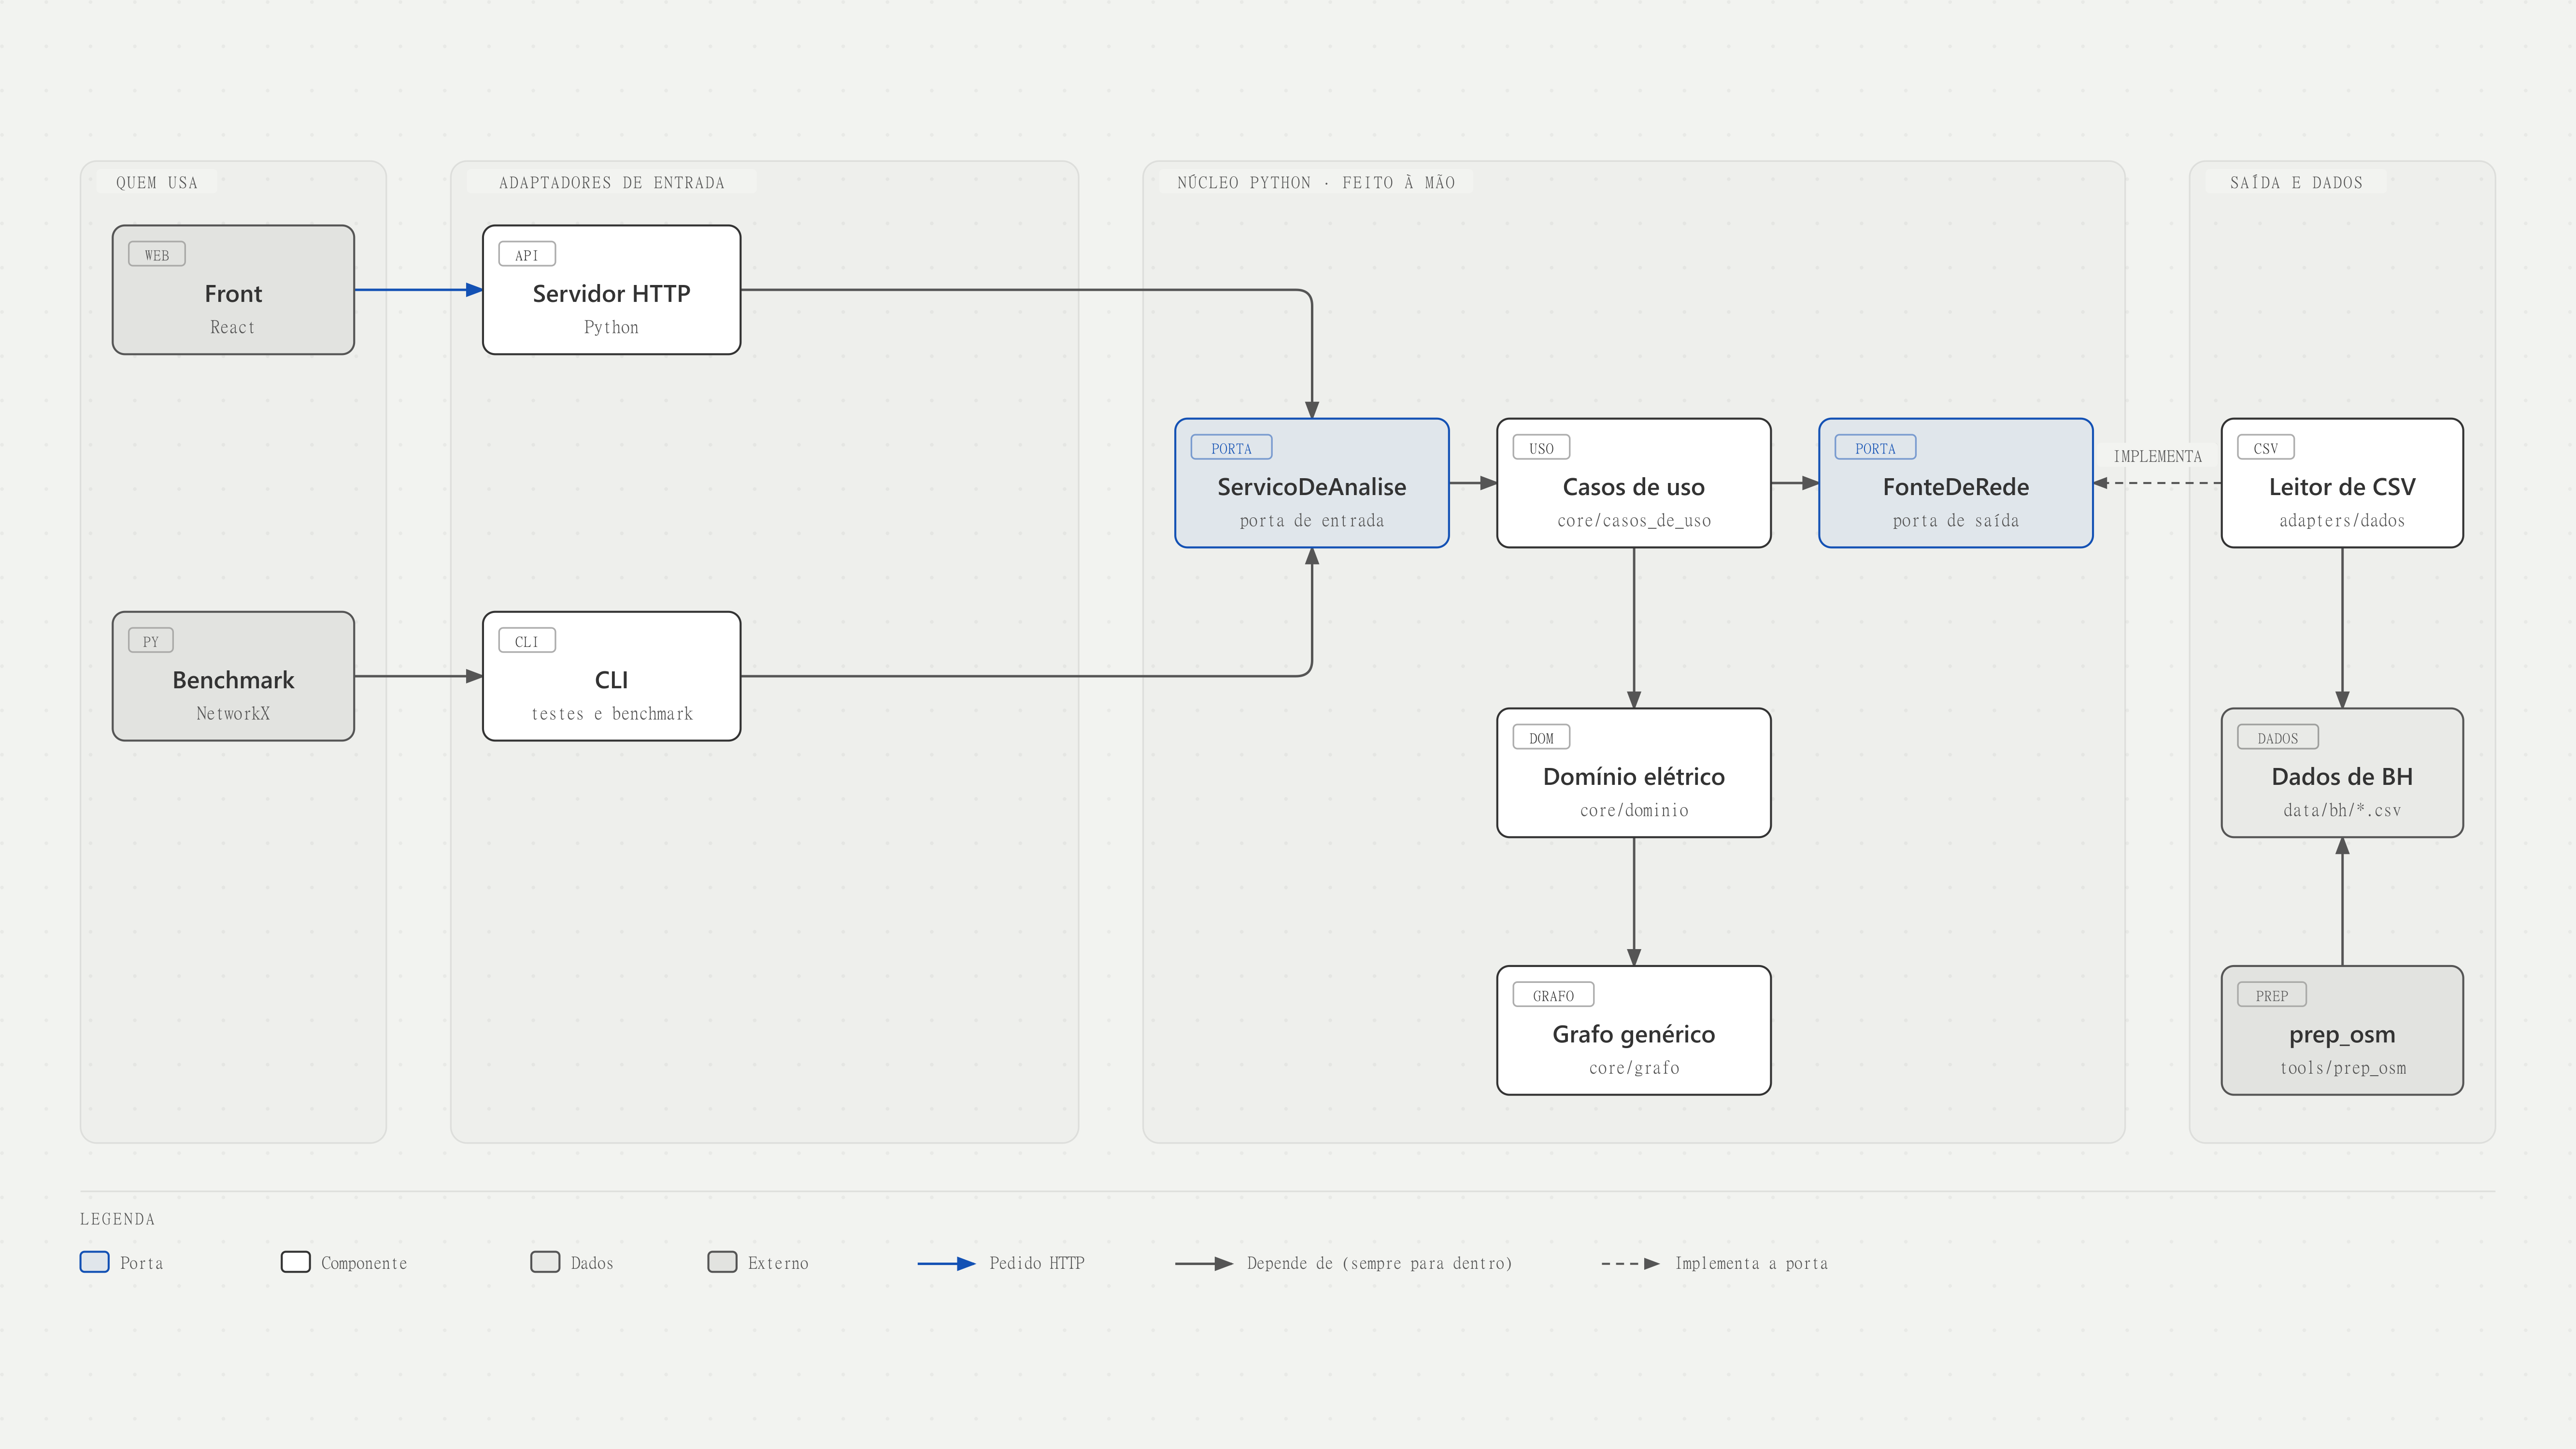
\includegraphics[width=.85\textwidth]{figuras/hexagono.png}
\caption{Arquitetura atual. O HTTP usa a porta ServicoDeAnalise; a CLI do benchmark, como ponto de montagem, chama os algoritmos genéricos diretamente. O leitor CSV implementa FonteDeRede.}
\label{fig:hexagono}
\end{figure}

Os casos de uso são \texttt{GerarRedeSintetica}, \texttt{CalcularFluxo}, \texttt{SimularFalha}, \texttt{PontosCriticos} e \texttt{RotaAlternativa}. A API é \textbf{sem estado}: o servidor carrega a rede uma vez, e cada pedido traz a lista completa de falhas e de chaves fechadas. Os cenários não alteram a rede armazenada, e cada cálculo cria seu próprio Dinic. O servidor mantém em memória o desenho da rede e a análise sem falhas, preparados ao ligar. Pedidos de análise com falhas e de rota entram em uma fila protegida por trava: um cálculo por vez; conexões canceladas enquanto esperavam são descartadas antes de chamar o núcleo. O campo tempoMs mede o cálculo e exclui a espera nessa fila. O contrato da API (rede, análise, rota alternativa e pontos críticos, em JSON) foi congelado no início do projeto, e o front foi desenvolvido em paralelo com arquivos de exemplo no mesmo formato.

Um \textbf{verificador} roda em hooks do git e no GitHub Actions em todo pedido de integração. Ele barra, entre outras coisas, o uso de biblioteca de grafo fora do benchmark, o uso de \texttt{heapq} no núcleo, dependências que apontam para fora do núcleo e commits na \texttt{main}.

\subsection{Telas e interação na versão atual}

O front usa React, MapLibre GL~\cite{maplibre} e deck.gl~\cite{deckgl}. A interface atual tem um console no topo com a marca REMG, energia entregue e demanda, gargalos, tempo do cálculo e situação da cidade. Os botões de tema e Camadas ficam no próprio console; zoom e bússola ficam no canto inferior, e a legenda de uso pode ser recolhida. Os painéis são superfícies sólidas: brancas no tema claro e azul-marinho no escuro, com tipografia Rawline e Raleway de reserva.

\begin{figure}[!htbp]
\centering
\begin{minipage}{.48\textwidth}\centering
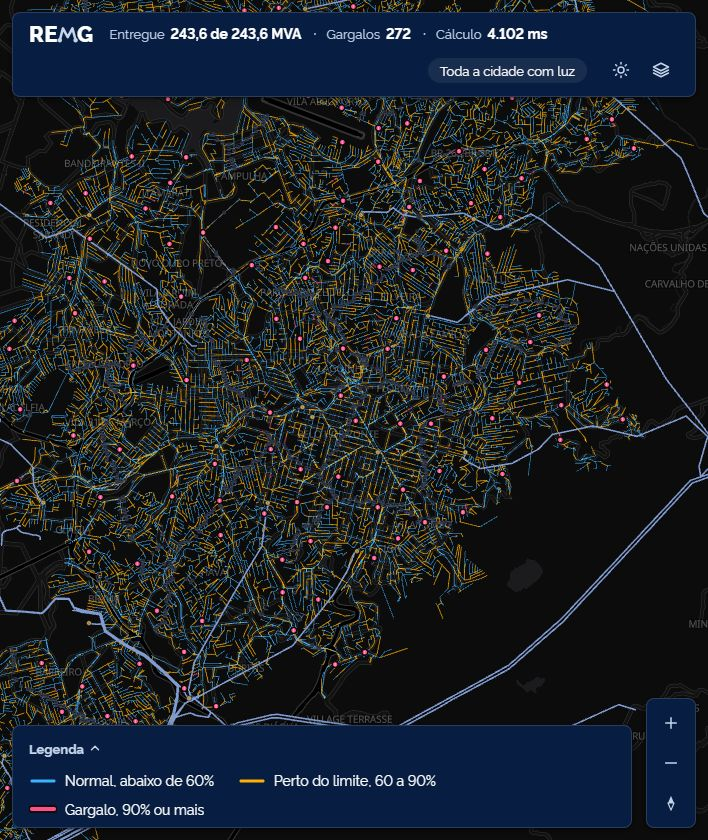
\includegraphics[width=\textwidth]{figuras/tela-atual-escura.jpg}
\end{minipage}\hfill
\begin{minipage}{.48\textwidth}\centering
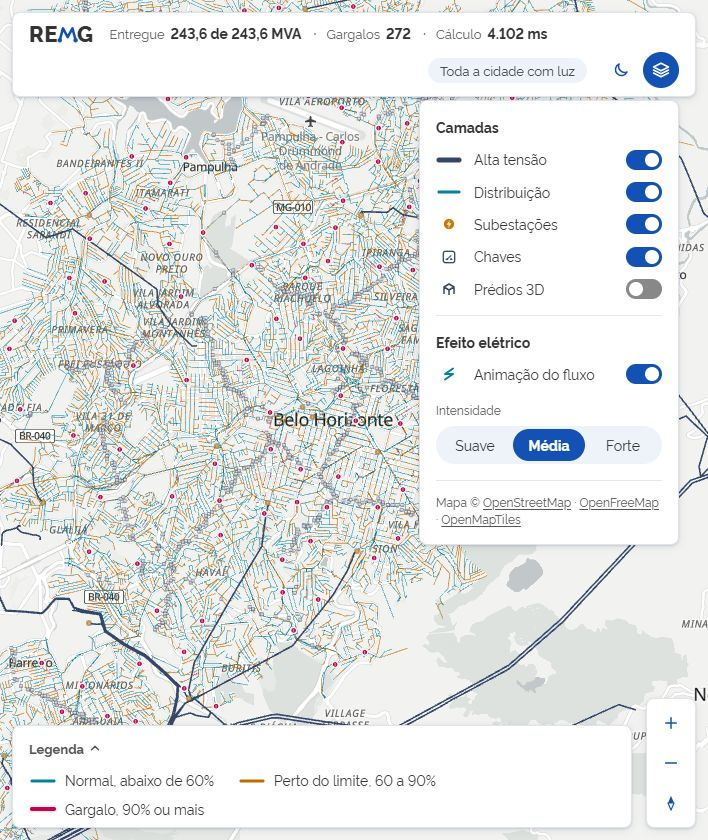
\includegraphics[width=\textwidth]{figuras/tela-camadas.jpg}
\end{minipage}
\caption{Capturas atuais ligadas ao servidor: à esquerda, tema escuro sem falhas; à direita, tema claro com o painel Camadas. O console mostra 243,6 de 243,6 MVA e 272 gargalos. Os tempos são os exibidos na sessão, não as medianas do benchmark.}
\label{fig:tela}
\end{figure}

As linhas são coloridas pelo uso: azul no escuro ou ciano no claro abaixo de 60\%, laranja de 60 a 90\% e rosa a partir de 90\%. Gargalos também recebem halo e marcador, e marcadores próximos são agrupados conforme o zoom. A animação acompanha o sentido do fluxo com ondas e, de perto, raios; o painel permite desligá-la e escolher intensidade suave, média ou forte. A preferência do sistema por movimento reduzido é respeitada. Alta tensão, distribuição, subestações e chaves podem ser exibidas separadamente. Há ainda prédios 3D derivados dos dados do mapa, visíveis a partir do zoom 15; eles não participam do grafo elétrico.

Clicar numa peça abre o cartão de detalhes com capacidade, estado e, quando aplicável, fluxo, uso e indicação de ponte ou articulação. O botão Derrubar acrescenta a peça à lista de falhas. A área desconectada aparece sem luz, e a lista permite restaurar um item ou todos. O botão Achar rota calcula as chaves a fechar, atualiza o fluxo e informa quantos pontos e quanta demanda foram religados, inclusive quando falta capacidade para atender tudo. Um novo pedido cancela a requisição anterior no navegador; os retornos antigos não substituem o cenário mais recente.

\begin{figure}[!htbp]
\centering
\begin{minipage}{.48\textwidth}\centering
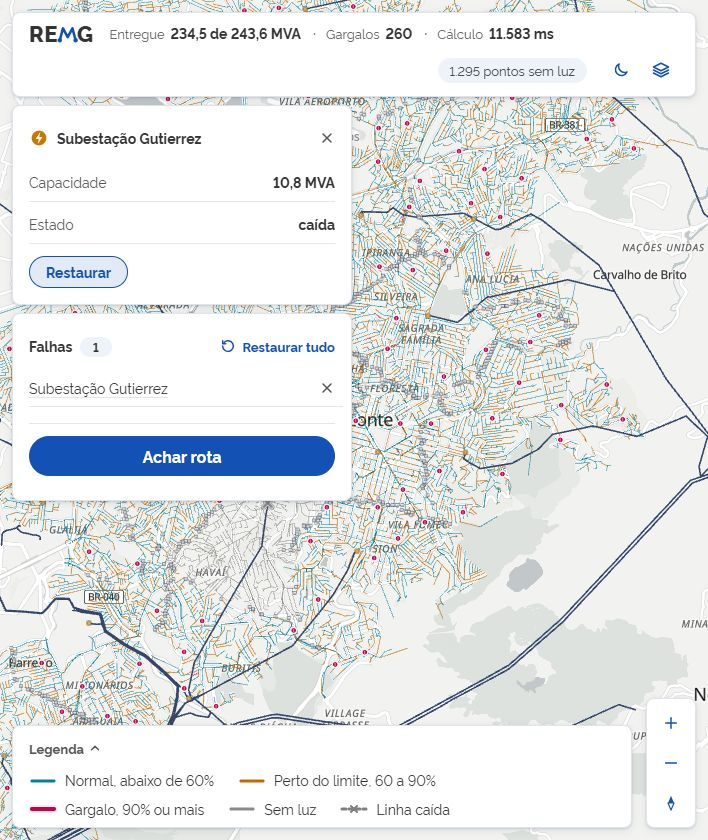
\includegraphics[width=\textwidth]{figuras/tela-falha-real.jpg}
\end{minipage}\hfill
\begin{minipage}{.48\textwidth}\centering
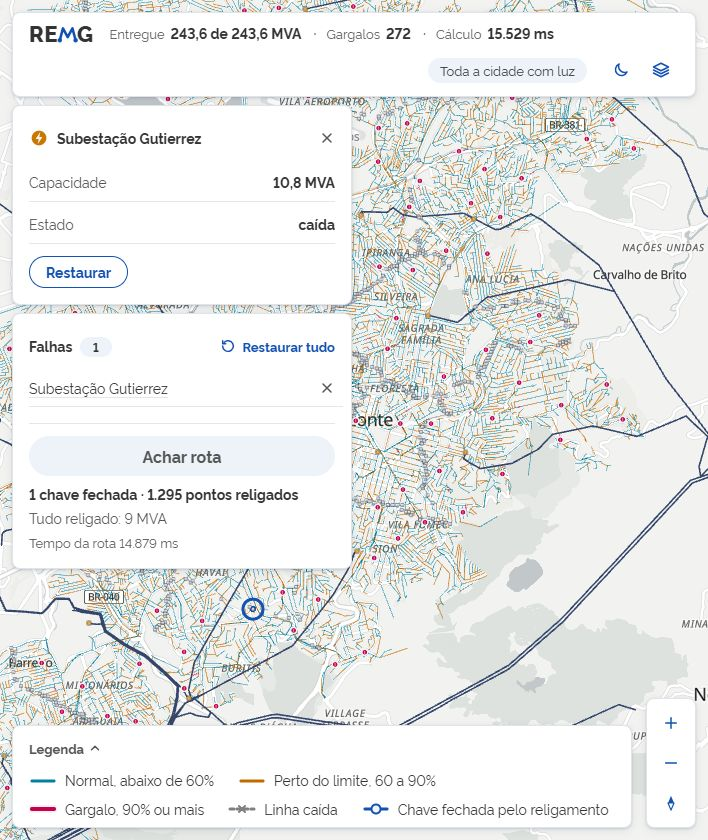
\includegraphics[width=\textwidth]{figuras/tela-religada-real.jpg}
\end{minipage}
\caption{Teste real pela interface: Gutierrez caída deixa 1.295 pontos sem luz (esquerda). Achar rota fecha uma chave e religa os 1.295 pontos (direita). O cartão da subestação continua indicando caída: o atendimento volta pelo caminho alternativo.}
\label{fig:telas-reais}
\end{figure}

\section{Resultados}
\label{sec:resultados}

O benchmark da Seção~\ref{sec:benchmark} foi executado em 22/11/2026, no Windows AMD64, com Python 3.13.14 e NetworkX 3.7. Nesta atualização, também foram conferidos diretamente nos CSV e no núcleo os dados da rede e os cenários de falha. As telas foram capturadas com VITE\_USAR\_MOCK=false e o servidor local ligado. O tempo exibido na interface, a duração da análise elétrica completa e a mediana do benchmark correspondem a medições distintas; variam com a carga da máquina.

\subsection{A rede de Belo Horizonte}
\label{sec:resultados-rede}

A rede foi montada novamente a partir dos CSV em 22/11/2026; as contagens abaixo foram confirmadas na execução atual. A Tabela~\ref{tab:rede} resume a rede obtida e a análise sem falhas.

\begin{table}[ht]
\centering
\caption{Rede gerada para Belo Horizonte e resultado da análise sem falhas.}
\label{tab:rede}
\begin{tabularx}{\textwidth}{Xr}
\toprule
\textbf{Medida} & \textbf{Valor} \\
\midrule
Subestações de distribuição & 18 \\
Subestações ligadas direto em $S$ (sem alta tensão no OSM) & 5 \\
Pontos de suprimento na divisa & 17 \\
Pontos na rede (fora: 702 sem rua até uma subestação) & 35.127 \\
Trechos de cabo / chaves de manobra & 35.109 / 827 \\
Grafo do fluxo: vértices / arcos & 35.164 / 142.244 \\
\midrule
Demanda total & 243.552,839 kVA \\
Fluxo máximo (energia entregue) & 243.552,839 kVA (100\%) \\
Arestas com fluxo & 35.122 \\
Gargalos (corte mínimo ou uso $\geq 90\%$) & 272 \\
Arestas com uso entre 60\% e 90\% / abaixo de 60\% & 13.442 / 21.408 \\
Tempo da análise elétrica completa (mediana de 3) & 9,1~s \\
Fluxo máximo só com Edmonds-Karp (benchmark) & não terminou em 120 s \\
\midrule
Pontos críticos com todas as chaves fechadas: pontes / articulações & 25.689 / 20.017 \\
\bottomrule
\end{tabularx}
\end{table}

Sem falhas, toda a demanda é atendida, porque nenhum cabo nasce menor que a carga que passa por ele (o menor fator é 1,1). Os 272 gargalos são os cabos com fator sorteado perto do mínimo, cujo uso passa de 90\%. O valor do fluxo do Dinic foi conferido com o do NetworkX no benchmark (Seção~\ref{sec:benchmark}). Mesmo com todas as chaves fechadas, a maior parte das arestas continua sendo ponte: as chaves (827) ficam só nas fronteiras entre as 18 áreas, e dentro de cada área a rede continua radial.

\textbf{Falhas.} Derrubar a subestação Pampulha, a de maior capacidade, deixa 6.727 pontos sem energia (46.684~kVA), e o fluxo cai para 196.869~kVA; o tempo da simulação depende da carga da máquina. Derrubar o trecho de maior capacidade da cidade (um tronco de 123.716~kVA) apaga 1.275 pontos (9.171~kVA). Nos dois casos, a rota alternativa fecha \textbf{uma chave} e religa toda a área. Derrubando cada uma das 18 subestações, uma por vez, 17 áreas voltam por completo; só a de Bonsucesso tem religamento \textbf{parcial} (Seção~\ref{sec:limitacoes}).

\subsection{Benchmark: núcleo $\times$ NetworkX}
\label{sec:benchmark}

O benchmark executa as rotinas do núcleo e as referências do NetworkX~3.7 sobre os mesmos dados. Foram usados grafos aleatórios de 1.000, 10.000 e 50.000 vértices, o grafo das ruas de Belo Horizonte e o grafo da rede elétrica. Os aleatórios usam semente 2026, grau médio 3, capacidades inteiras de 1 a 100 e pesos de 1 a 500. Cada caso é gerado uma vez; os dois lados recebem as mesmas arestas, capacidades, pesos e, no fluxo, os mesmos terminais $S$ e $T$. O Dijkstra comparado parte apenas do vértice 0.

Os tempos são medianas de três rodadas. A leitura do arquivo, a montagem inicial do grafo e a inicialização do processo Python ficam fora da medição. O intervalo cronometrado inclui a rotina chamada e a preparação de seus resultados; esse trabalho não é idêntico nos dois lados. A Tabela~\ref{tab:bench} mostra uma seleção dos 28 pares previstos: 27 terminaram e tiveram respostas iguais; o Edmonds-Karp na rede elétrica excedeu 120~s em uma rodada do núcleo, e o NetworkX não foi medido nesse par. A razão é o tempo do núcleo dividido pelo do NetworkX.

\begin{table}[ht]
\centering
\caption{Benchmark de 22/11/2026 (ms, mediana de 3 rodadas). Respostas iguais nos casos concluídos. As linhas de fluxo usam preflow-push como referência no NetworkX.}
\label{tab:bench}
\small\setlength{\tabcolsep}{4pt}
\begin{tabularx}{\textwidth}{Xlrrr}
\toprule
\textbf{Grafo ($V$ / $E$)} & \textbf{Algoritmo} & \textbf{Núcleo} & \textbf{NetworkX} & \textbf{Razão} \\
\midrule
aleatório (10.000 / 15.000) & Dinic & 33,73 & 411,99 & 0,08 \\
 & Edmonds-Karp & 143,52 & 435,61 & 0,33 \\
 & Dijkstra & 35,45 & 52,41 & 0,68 \\
 & pontes (Tarjan) & 9,03 & 419,80 & 0,02 \\
 & Kruskal & 19,98 & 137,51 & 0,15 \\
\midrule
aleatório (50.000 / 75.000) & Dinic & 600,14 & 1.409,00 & 0,43 \\
 & Edmonds-Karp & 1.209,94 & 1.477,43 & 0,82 \\
 & componentes (BFS) & 50,55 & 43,89 & 1,15 \\
 & articulações (Tarjan) & 68,58 & 114,87 & 0,60 \\
\midrule
BH ruas (35.829 / 53.230) & Dijkstra & 75,36 & 79,29 & 0,95 \\
 & componentes (BFS) & 12,22 & 13,77 & 0,89 \\
 & pontes (Tarjan) & 26,38 & 607,09 & 0,04 \\
 & articulações (Tarjan) & 31,68 & 77,35 & 0,41 \\
 & Kruskal & 79,31 & 648,33 & 0,12 \\
\midrule
BH rede elétrica (35.164 / 71.122) & Dinic & 3.723,73 & 10.768,41 & 0,35 \\
 & Edmonds-Karp & \multicolumn{3}{c}{núcleo >120 s; NX não medido} \\
\bottomrule
\end{tabularx}
\end{table}

O núcleo foi mais rápido em 25 dos 27 casos concluídos. As exceções foram Dijkstra e BFS no grafo de 50.000 vértices, com tempos cerca de 16\% e 15\% maiores, respectivamente. Para pontes, a vantagem observada variou de aproximadamente 13 a 46 vezes. No grafo aleatório de 1.000 vértices, Edmonds-Karp levou 1,26~ms e Dinic, 3,51~ms. Na rede elétrica de BH, Dinic levou 3.723,73~ms, contra 10.768,41~ms da referência, enquanto Edmonds-Karp excedeu o limite de 120~s. Nesse cenário, a medição favorece o uso do Dinic entre as duas implementações do núcleo.

\textbf{Algoritmo de referência.} As duas linhas de fluxo chamam \texttt{maximum\_flow\_value} sem definir \texttt{flow\_func}. Na versão 3.7 instalada, a função usa \texttt{preflow\_push}. Portanto, essas linhas comparam Dinic e Edmonds-Karp com outra estratégia para resolver o mesmo problema; não medem Dinic contra Dinic nem Edmonds-Karp contra Edmonds-Karp. As arestas paralelas são preservadas em um multigrafo para os demais problemas; no fluxo, suas capacidades são somadas, pois a função de referência não aceita multigrafos.

\textbf{Alcance da conferência.} São comparados o valor total do fluxo, as distâncias, os componentes, as pontes, as articulações e o custo e o número de componentes da floresta mínima. A conferência não valida a distribuição do fluxo por aresta nem o corte mínimo. Distâncias e custos usam tolerância relativa de $10^{-6}$, com escala mínima 1; os demais resultados usam igualdade exata. A igualdade observada vale para os casos executados.

\textbf{Capacidade zero e falhas.} BFS e Tarjan do núcleo ignoram arestas de capacidade zero; as referências de conectividade do benchmark mantêm essas arestas. Um caso adicional com dois vértices ligados por uma aresta de capacidade zero confirmou a diferença: o núcleo encontrou dois componentes e nenhuma ponte; o NetworkX encontrou um componente e uma ponte. Os casos de conectividade desta execução têm capacidades positivas, e a rede elétrica foi usada apenas para fluxo. Assim, o benchmark atual não verifica a equivalência das regras de falha e religamento. Os cinco testes existentes da ferramenta de benchmark também passaram nesta revisão.

% =====================================================================
\section{Limitações}
\label{sec:limitacoes}

\begin{itemize}
  \item \textbf{Fluxo máximo não é física elétrica.} No modelo, a energia \textquotedblleft{}escolhe\textquotedblright{} o caminho que maximiza a entrega. Na rede real, quem decide é a impedância dos cabos, e entram tensão, potência reativa e perdas. O sistema responde a perguntas de capacidade e de conectividade, não de fluxo de carga.
  \item \textbf{A distribuição é sintética.} Os traçados seguem as ruas reais, mas a demanda (proporcional ao comprimento de rua) e as capacidades (com fator sorteado) são modelos, não dados da concessionária. Os gargalos encontrados são do modelo, não da cidade.
  \item \textbf{Socorro dimensionado para uma falha por vez.} Só a chave de socorro de cada área e o caminho até as raízes recebem folga para a área vizinha. Com uma subestação caída, 17 das 18 áreas voltam por completo, mas a de Bonsucesso volta só em parte, e falhas simultâneas em áreas vizinhas podem não ter caminho com capacidade suficiente.
  \item \textbf{Alta tensão incompleta.} Cinco subestações não têm linha de alta tensão no OSM e foram ligadas direto à super-fonte; nelas, derrubar uma linha de alta tensão não tem efeito.
\end{itemize}

% =====================================================================
\section{Processo, uso de IA e responsabilidades}
\label{sec:processo}

\subsection{Processo de trabalho}

O trabalho foi dividido em cerca de 30 tarefas, cada uma com um arquivo de descrição e uma issue no GitHub, organizadas num quadro kanban e em versões com data-alvo (v0.1 Base até v1.0 Entrega). Cada tarefa tem uma branch própria, e a integração na \texttt{main} só acontece por pedido de integração revisado por um colega e com o verificador aprovado, com \emph{merge} sem \emph{squash} para preservar os commits individuais. As decisões de projeto foram registradas com data e justificativa (27 decisões numeradas).

\subsection{Uso de inteligência artificial}

O grupo usou assistentes de IA (Claude Code e Codex) como ferramenta de apoio: no planejamento da especificação e das tarefas, nas automações do repositório e no verificador, no front, na extração dos dados do OSM, na revisão de código e na redação e revisão deste relatório. As regras do projeto valem também para a IA: um arquivo de instruções na raiz do repositório (\texttt{AGENTS.md}) e uma guarda no Claude Code a impedem de pular o verificador e de usar biblioteca de grafos no núcleo.

As decisões foram do grupo: o tema, a cidade inteira em vez de uma única regional (sugestão inicial da IA), a arquitetura hexagonal, a escolha do Dinic apoiada pelas medições e o escopo do trabalho. Sugestões da IA foram aceitas quando ajudavam (por exemplo, o contrato sem estado da API) e recusadas quando não serviam, como vários efeitos visuais propostos para o mapa. A IA também errou em pontos que só os testes revelaram, como números incoerentes num arquivo de exemplo; por isso todos os números deste relatório vêm de execução real. Todo código entrou por pedido de integração revisado por um colega, e cada integrante apresenta a própria parte no vídeo.

\subsection{Responsabilidades}

A Tabela~\ref{tab:membros} resume o que cada integrante fez, segundo as issues e o histórico de commits.

\begin{table}[ht]
\centering
\caption{Responsabilidades de cada integrante.}
\label{tab:membros}
\begin{tabularx}{\textwidth}{lX}
\toprule
\textbf{Integrante} & \textbf{Principais entregas} \\
\midrule
Davi Lage & leitor dos CSV (porta \texttt{FonteDeRede}); benchmark do núcleo contra o NetworkX; revisão e integração de pedidos; relatório \\
Isaias Alves & heap binária e Dijkstra com várias fontes; geração da rede sintética; cálculo de fluxo e gargalos; simulação de falha; Tarjan iterativo e pontos críticos; linha de comando; plano B da alta tensão \\
Laura Noronha Lara & estrutura do grafo e BFS; Dinic e corte mínimo; slides; \texttt{RedeEletrica}; Edmonds-Karp; Kruskal e \emph{union-find}; rota alternativa; Edmonds-Karp e Kruskal na linha de comando; relatório \\
Lucas Spiazzi & revisão da arquitetura e contrato da API; direção visual e protótipo; repositório, verificador e automação do fluxo; extração do OSM; front (base, camadas, animação, derrubar e religar); servidor; regra de socorro da rede sintética; UML \\
\bottomrule
\end{tabularx}
\end{table}

% =====================================================================
\section{Conclusão}
\label{sec:conclusao}

O REMG mostra que as perguntas de operação de uma rede de distribuição de energia (quanto chega, onde trava, quem apaga e como religar) se traduzem diretamente em fluxo máximo, corte mínimo, busca em largura, caminhos mínimos e pontes. Aplicados à cidade inteira de Belo Horizonte, com mais de 35 mil vértices, esses algoritmos, escritos à mão em Python puro, deram as mesmas respostas que o NetworkX e foram mais rápidos que ele na maior parte dos casos. Entre as duas implementações de fluxo do núcleo, o Dinic teve melhor desempenho na rede elétrica: na rede da cidade ele levou cerca de 3,72~s no benchmark, enquanto o Edmonds-Karp excedeu o limite de 120~s em uma rodada.

A modelagem com super-fonte, super-sorvedouro e capacidade zero para falhas e chaves abertas permitiu responder a todas as perguntas sobre o mesmo grafo, só trocando capacidades. A arquitetura hexagonal separou o núcleo de grafos do domínio elétrico e dos adaptadores, o que deixou o núcleo testável sozinho e permitiu que o front fosse desenvolvido em paralelo.

Como trabalhos futuros, ficam: dimensionar a rede para falhas simultâneas, e não só para a queda de uma subestação por vez; a expansão para a região metropolitana, que já é um parâmetro da extração de dados; e o uso do Kruskal na própria tela, para sugerir onde instalar novos cabos com o menor custo.

\bibliographystyle{sbc}
\bibliography{relatorio}

\end{document}